%%%%%%%%%%%%%%%%%%%%%%%%%%%%%%%%%%%%%%%%%
%  My documentation report
%  Objetive: Explain what I did and how, so someone can continue with the investigation
%
% Important note:
% Chapter heading images should have a 2:1 width:height ratio,
% e.g. 920px width and 460px height.
%
%%%%%%%%%%%%%%%%%%%%%%%%%%%%%%%%%%%%%%%%%


%----------------------------------------------------------------------------------------
%	PACKAGES AND OTHER DOCUMENT CONFIGURATIONS
%----------------------------------------------------------------------------------------

\documentclass[11pt,fleqn]{book} % Default font size and left-justified equations


\usepackage[top=3cm,bottom=3cm,left=3.2cm,right=3.2cm,headsep=10pt,letterpaper]{geometry} % Page margins

\usepackage{xcolor} % Required for specifying colors by name
\definecolor{ocre}{RGB}{52,177,201} % Define the orange color used for highlighting throughout the book

% Font Settings
\usepackage{avant} % Use the Avantgarde font for headings
%\usepackage{times} % Use the Times font for headings
\usepackage{mathptmx} % Use the Adobe Times Roman as the default text font together with math symbols from the Sym­bol, Chancery and Com­puter Modern fonts
\usepackage{microtype} % Slightly tweak font spacing for aesthetics
\usepackage[utf8]{inputenc} % Required for including letters with accents
\usepackage[T1]{fontenc} % Use 8-bit encoding that has 256 glyphs
\usepackage{amsthm}

% Bibliography
%\usepackage[style=alphabetic,sorting=nyt,sortcites=true,autopunct=true,babel=hyphen,hyperref=true,abbreviate=false,backref=true,backend=biber]{biblatex}
%\addbibresource{bio.bib} % BibTeX bibliography file
%\defbibheading{bibempty}{}

%----------------------------------------------------------------------------------------
%	VARIOUS REQUIRED PACKAGES
%----------------------------------------------------------------------------------------

\usepackage{titlesec} % Allows customization of titles

\usepackage{graphicx} % Required for including pictures
\graphicspath{{Pictures/}} % Specifies the directory where pictures are stored
% \graphicspath{{Plots/}}
\usepackage{lipsum} % Inserts dummy text

\usepackage{tikz} % Required for drawing custom shapes

\usepackage[spanish]{babel} % English language/hyphenation

\usepackage{enumitem} % Customize lists
\setlist{nolistsep} % Reduce spacing between bullet points and numbered lists

\usepackage{booktabs} % Required for nicer horizontal rules in tables

\usepackage{eso-pic} % Required for specifying an image background in the title page


\usepackage[ruled,vlined,lined]{algorithm2e}
\usepackage{listings}


%----------------------------------------------------------------------------------------
%	MAIN TABLE OF CONTENTS
%----------------------------------------------------------------------------------------

\usepackage{titletoc} % Required for manipulating the table of contents

\contentsmargin{0cm} % Removes the default margin
% Chapter text styling
\titlecontents{chapter}[1.25cm] % Indentation
{\addvspace{15pt}\large\sffamily\bfseries} % Spacing and font options for chapters
{\color{ocre!60}\contentslabel[\Large\thecontentslabel]{1.25cm}\color{ocre}} % Chapter number
{}  
{\color{ocre!60}\normalsize\sffamily\bfseries\;\titlerule*[.5pc]{.}\;\thecontentspage} % Page number
% Section text styling
\titlecontents{section}[1.25cm] % Indentation
{\addvspace{5pt}\sffamily\bfseries} % Spacing and font options for sections
{\contentslabel[\thecontentslabel]{1.25cm}} % Section number
{}
{\sffamily\hfill\color{black}\thecontentspage} % Page number
[]
% Subsection text styling
\titlecontents{subsection}[1.25cm] % Indentation
{\addvspace{1pt}\sffamily\small} % Spacing and font options for subsections
{\contentslabel[\thecontentslabel]{1.25cm}} % Subsection number
{}
{\sffamily\;\titlerule*[.5pc]{.}\;\thecontentspage} % Page number
[] 

%----------------------------------------------------------------------------------------
%	MINI TABLE OF CONTENTS IN CHAPTER HEADS
%----------------------------------------------------------------------------------------

% Section text styling
\titlecontents{lsection}[0em] % Indendating
{\footnotesize\sffamily} % Font settings
{}
{}
{}

% Subsection text styling
\titlecontents{lsubsection}[.5em] % Indentation
{\normalfont\footnotesize\sffamily} % Font settings
{}
{}
{}
 
%----------------------------------------------------------------------------------------
%	PAGE HEADERS
%----------------------------------------------------------------------------------------

\usepackage{fancyhdr} % Required for header and footer configuration

\pagestyle{fancy}
\renewcommand{\chaptermark}[1]{\markboth{\sffamily\normalsize\bfseries\chaptername\ \thechapter.\ #1}{}} % Chapter text font settings
\renewcommand{\sectionmark}[1]{\markright{\sffamily\normalsize\thesection\hspace{5pt}#1}{}} % Section text font settings
\fancyhf{} \fancyhead[LE,RO]{\sffamily\normalsize\thepage} % Font setting for the page number in the header
\fancyhead[LO]{\rightmark} % Print the nearest section name on the left side of odd pages
\fancyhead[RE]{\leftmark} % Print the current chapter name on the right side of even pages
\renewcommand{\headrulewidth}{0.5pt} % Width of the rule under the header
\addtolength{\headheight}{2.5pt} % Increase the spacing around the header slightly
\renewcommand{\footrulewidth}{0pt} % Removes the rule in the footer
\fancypagestyle{plain}{\fancyhead{}\renewcommand{\headrulewidth}{0pt}} % Style for when a plain pagestyle is specified

% Removes the header from odd empty pages at the end of chapters
\makeatletter
\renewcommand{\cleardoublepage}{
\clearpage\ifodd\c@page\else
\hbox{}
\vspace*{\fill}
\thispagestyle{empty}
\newpage
\fi}

%----------------------------------------------------------------------------------------
%	THEOREM STYLES
%----------------------------------------------------------------------------------------

\usepackage{amsmath,amsfonts,amssymb,amsthm} % For math equations, theorems, symbols, etc

\newcommand{\intoo}[2]{\mathopen{]}#1\,;#2\mathclose{[}}
\newcommand{\ud}{\mathop{\mathrm{{}d}}\mathopen{}}
\newcommand{\intff}[2]{\mathopen{[}#1\,;#2\mathclose{]}}
\newtheorem{notation}{Notation}[chapter]

%%%%%%%%%%%%%%%%%%%%%%%%%%%%%%%%%%%%%%%%%%%%%%%%%%%%%%%%%%%%%%%%%%%%%%%%%%%
%%%%%%%%%%%%%%%%%%%% dedicated to boxed/framed environements %%%%%%%%%%%%%%
%%%%%%%%%%%%%%%%%%%%%%%%%%%%%%%%%%%%%%%%%%%%%%%%%%%%%%%%%%%%%%%%%%%%%%%%%%%
\newtheoremstyle{ocrenumbox}% % Theorem style name
{0pt}% Space above
{0pt}% Space below
{\normalfont}% % Body font
{}% Indent amount
{\small\bf\sffamily\color{ocre}}% % Theorem head font
{\;}% Punctuation after theorem head
{0.25em}% Space after theorem head
{\small\sffamily\color{ocre}\thmname{#1}\nobreakspace\thmnumber{\@ifnotempty{#1}{}\@upn{#2}}% Theorem text (e.g. Theorem 2.1)
\thmnote{\nobreakspace\the\thm@notefont\sffamily\bfseries\color{black}---\nobreakspace#3.}} % Optional theorem note
\renewcommand{\qedsymbol}{$\blacksquare$}% Optional qed square

\newtheoremstyle{blacknumex}% Theorem style name
{5pt}% Space above
{5pt}% Space below
{\normalfont}% Body font
{} % Indent amount
{\small\bf\sffamily}% Theorem head font
{\;}% Punctuation after theorem head
{0.25em}% Space after theorem head
{\small\sffamily{\tiny\ensuremath{\blacksquare}}\nobreakspace\thmname{#1}\nobreakspace\thmnumber{\@ifnotempty{#1}{}\@upn{#2}}% Theorem text (e.g. Theorem 2.1)
\thmnote{\nobreakspace\the\thm@notefont\sffamily\bfseries---\nobreakspace#3.}}% Optional theorem note

\newtheoremstyle{blacknumbox} % Theorem style name
{0pt}% Space above
{0pt}% Space below
{\normalfont}% Body font
{}% Indent amount
{\small\bf\sffamily}% Theorem head font
{\;}% Punctuation after theorem head
{0.25em}% Space after theorem head
{\small\sffamily\thmname{#1}\nobreakspace\thmnumber{\@ifnotempty{#1}{}\@upn{#2}}% Theorem text (e.g. Theorem 2.1)
\thmnote{\nobreakspace\the\thm@notefont\sffamily\bfseries---\nobreakspace#3.}}% Optional theorem note

%%%%%%%%%%%%%%%%%%%%%%%%%%%%%%%%%%%%%%%%%%%%%%%%%%%%%%%%%%%%%%%%%%%%%%%%%%%
%%%%%%%%%%%%% dedicated to non-boxed/non-framed environements %%%%%%%%%%%%%
%%%%%%%%%%%%%%%%%%%%%%%%%%%%%%%%%%%%%%%%%%%%%%%%%%%%%%%%%%%%%%%%%%%%%%%%%%%
\newtheoremstyle{ocrenum}% % Theorem style name
{5pt}% Space above
{5pt}% Space below
{\normalfont}% % Body font
{}% Indent amount
{\small\bf\sffamily\color{ocre}}% % Theorem head font
{\;}% Punctuation after theorem head
{0.25em}% Space after theorem head
{\small\sffamily\color{ocre}\thmname{#1}\nobreakspace\thmnumber{\@ifnotempty{#1}{}\@upn{#2}}% Theorem text (e.g. Theorem 2.1)
\thmnote{\nobreakspace\the\thm@notefont\sffamily\bfseries\color{black}---\nobreakspace#3.}} % Optional theorem note
\renewcommand{\qedsymbol}{$\blacksquare$}% Optional qed square
\makeatother

% Defines the theorem text style for each type of theorem to one of the three styles above
\newcounter{dummy} 
\numberwithin{dummy}{section}
\theoremstyle{ocrenumbox}


\newtheorem{theoremeT}[dummy]{Theorem}
\newtheorem{lemma}[dummy]{Lemma}
\newtheorem{observation}[dummy]{Observation}
\newtheorem{proposition}[dummy]{Proposition}
% \newtheorem{definition}[dummy]{Definition}
\newtheorem{claim}[dummy]{Claim}
\newtheorem{fact}[dummy]{Fact}
\newtheorem{assumption}[dummy]{Assumption}

\newtheorem{problem}{Problem}[chapter]
% \newtheorem{exercise}{Exercise}[chapter]
\theoremstyle{blacknumex}
\newtheorem{exampleT}{Ejemplo}[chapter]
\theoremstyle{blacknumbox}
\newtheorem{vocabulary}{Vocabulary}[chapter]
\newtheorem{definitionT}{Definición}[section]
\newtheorem{corollaryT}[dummy]{Corollary}
\theoremstyle{ocrenum}

%----------------------------------------------------------------------------------------
%	DEFINITION OF COLORED BOXES
%----------------------------------------------------------------------------------------

\RequirePackage[framemethod=default]{mdframed} % Required for creating the theorem, definition, exercise and corollary boxes

% Theorem box
\newmdenv[skipabove=7pt,
skipbelow=7pt,
backgroundcolor=black!5,
linecolor=ocre,
innerleftmargin=5pt,
innerrightmargin=5pt,
innertopmargin=5pt,
leftmargin=0cm,
rightmargin=0cm,
innerbottommargin=5pt]{tBox}

% Exercise box	  
\newmdenv[skipabove=7pt,
skipbelow=7pt,
rightline=false,
leftline=true,
topline=false,
bottomline=false,
backgroundcolor=ocre!10,
linecolor=ocre,
innerleftmargin=5pt,
innerrightmargin=5pt,
innertopmargin=5pt,
innerbottommargin=5pt,
leftmargin=0cm,
rightmargin=0cm,
linewidth=4pt]{eBox}	

% Definition box
\newmdenv[skipabove=7pt,
skipbelow=7pt,
rightline=false,
leftline=true,
topline=false,
bottomline=false,
linecolor=ocre,
innerleftmargin=5pt,
innerrightmargin=5pt,
innertopmargin=0pt,
leftmargin=0cm,
rightmargin=0cm,
linewidth=4pt,
innerbottommargin=0pt]{dBox}	

% Corollary box
\newmdenv[skipabove=7pt,
skipbelow=7pt,
rightline=false,
leftline=true,
topline=false,
bottomline=false,
linecolor=gray,
backgroundcolor=black!5,
innerleftmargin=5pt,
innerrightmargin=5pt,
innertopmargin=5pt,
leftmargin=0cm,
rightmargin=0cm,
linewidth=4pt,
innerbottommargin=5pt]{cBox}

% Creates an environment for each type of theorem and assigns it a theorem text style from the "Theorem Styles" section above and a colored box from above
\newenvironment{theorem}{\begin{tBox}\begin{theoremeT}}{\end{theoremeT}\end{tBox}}
\newenvironment{exercise}{\begin{eBox}\begin{exerciseT}}{\hfill{\color{ocre}\tiny\ensuremath{\blacksquare}}\end{exerciseT}\end{eBox}}				  
\newenvironment{definition}{\begin{dBox}\begin{definitionT}}{\end{definitionT}\end{dBox}}	
\newenvironment{example}{\begin{exampleT}}{\hfill{\tiny\ensuremath{\blacksquare}}\end{exampleT}}		
\newenvironment{corollary}{\begin{cBox}\begin{corollaryT}}{\end{corollaryT}\end{cBox}}	

%----------------------------------------------------------------------------------------
%	REMARK ENVIRONMENT
%----------------------------------------------------------------------------------------

\newenvironment{remark}{\par\vspace{10pt}\small % Vertical white space above the remark and smaller font size
\begin{list}{}{
\leftmargin=35pt % Indentation on the left
\rightmargin=25pt}\item\ignorespaces % Indentation on the right
\makebox[-2.5pt]{\begin{tikzpicture}[overlay]
\node[draw=ocre!60,line width=1pt,circle,fill=ocre!25,font=\sffamily\bfseries,inner sep=2pt,outer sep=0pt] at (-15pt,0pt){\textcolor{ocre}{R}};\end{tikzpicture}} % Orange R in a circle
\advance\baselineskip -1pt}{\end{list}\vskip5pt} % Tighter line spacing and white space after remark

%----------------------------------------------------------------------------------------
%	SECTION NUMBERING IN THE MARGIN
%----------------------------------------------------------------------------------------

\makeatletter
\renewcommand{\@seccntformat}[1]{\llap{\textcolor{ocre}{\csname the#1\endcsname}\hspace{1em}}}                    
\renewcommand{\section}{\@startsection{section}{1}{\z@}
{-4ex \@plus -1ex \@minus -.4ex}
{1ex \@plus.2ex }
{\normalfont\large\sffamily\bfseries}}
\renewcommand{\subsection}{\@startsection {subsection}{2}{\z@}
{-3ex \@plus -0.1ex \@minus -.4ex}
{0.5ex \@plus.2ex }
{\normalfont\sffamily\bfseries}}
\renewcommand{\subsubsection}{\@startsection {subsubsection}{3}{\z@}
{-2ex \@plus -0.1ex \@minus -.2ex}
{.2ex \@plus.2ex }
{\normalfont\small\sffamily\bfseries}}                        
\renewcommand\paragraph{\@startsection{paragraph}{4}{\z@}
{-2ex \@plus-.2ex \@minus .2ex}
{.1ex}
{\normalfont\small\sffamily\bfseries}}

%----------------------------------------------------------------------------------------
%	HYPERLINKS IN THE DOCUMENTS
%----------------------------------------------------------------------------------------

% For an unclear reason, the package should be loaded now and not later
\usepackage{hyperref}
\hypersetup{hidelinks,backref=true,pagebackref=true,hyperindex=true,colorlinks=false,breaklinks=true,urlcolor= ocre,bookmarks=true,bookmarksopen=false,pdftitle={Title},pdfauthor={Author}}

%----------------------------------------------------------------------------------------
%	CHAPTER HEADINGS
%----------------------------------------------------------------------------------------

% The set-up below should be (sadly) manually adapted to the overall margin page septup controlled by the geometry package loaded in the main.tex document. It is possible to implement below the dimensions used in the goemetry package (top,bottom,left,right)... TO BE DONE

\newcommand{\thechapterimage}{}
\newcommand{\chapterimage}[1]{\renewcommand{\thechapterimage}{#1}}

% Numbered chapters with mini tableofcontents
\def\thechapter{\arabic{chapter}}
\def\@makechapterhead#1{
\thispagestyle{empty}
{\centering \normalfont\sffamily
\ifnum \c@secnumdepth >\m@ne
\if@mainmatter
\startcontents
\begin{tikzpicture}[remember picture,overlay]
\node at (current page.north west)
{\begin{tikzpicture}[remember picture,overlay]
\node[anchor=north west,inner sep=0pt] at (0,0) {\includegraphics[width=\paperwidth]{\thechapterimage}};
%%%%%%%%%%%%%%%%%%%%%%%%%%%%%%%%%%%%%%%%%%%%%%%%%%%%%%%%%%%%%%%%%%%%%%%%%%%%%%%%%%%%%
% Commenting the 3 lines below removes the small contents box in the chapter heading
%\fill[color=ocre!10!white,opacity=.6] (1cm,0) rectangle (8cm,-7cm);
%\node[anchor=north west] at (1.1cm,.35cm) {\parbox[t][8cm][t]{6.5cm}{\huge\bfseries\flushleft \printcontents{l}{1}{\setcounter{tocdepth}{2}}}};
\draw[anchor=west] (5cm,-9cm) node [rounded corners=20pt,fill=ocre!10!white,text opacity=1,draw=ocre,draw opacity=1,line width=1.5pt,fill opacity=.6,inner sep=12pt]{\huge\sffamily\bfseries\textcolor{black}{\thechapter. #1\strut\makebox[22cm]{}}};
%%%%%%%%%%%%%%%%%%%%%%%%%%%%%%%%%%%%%%%%%%%%%%%%%%%%%%%%%%%%%%%%%%%%%%%%%%%%%%%%%%%%%
\end{tikzpicture}};
\end{tikzpicture}}
\par\vspace*{230\p@}
\fi
\fi}

% Unnumbered chapters without mini tableofcontents (could be added though) 
\def\@makeschapterhead#1{
\thispagestyle{empty}
{\centering \normalfont\sffamily
\ifnum \c@secnumdepth >\m@ne
\if@mainmatter
\begin{tikzpicture}[remember picture,overlay]
\node at (current page.north west)
{\begin{tikzpicture}[remember picture,overlay]
\node[anchor=north west,inner sep=0pt] at (0,0) {\includegraphics[width=\paperwidth]{\thechapterimage}};
\draw[anchor=west] (5cm,-9cm) node [rounded corners=20pt,fill=ocre!10!white,fill opacity=.6,inner sep=12pt,text opacity=1,draw=ocre,draw opacity=1,line width=1.5pt]{\huge\sffamily\bfseries\textcolor{black}{#1\strut\makebox[22cm]{}}};
\end{tikzpicture}};
\end{tikzpicture}}
\par\vspace*{230\p@}
\fi
\fi
}
\makeatother
 % Insert the commands.tex file which contains the majority of the structure behind the template

%----------------------------------------------------------------------------------------
%	Definitions of new commands
%----------------------------------------------------------------------------------------

\def\R{\mathbb{R}}
\newcommand{\cvx}{convex}
\begin{document}

%----------------------------------------------------------------------------------------
%	TITLE PAGE
%----------------------------------------------------------------------------------------

\begingroup
\thispagestyle{empty}
\AddToShipoutPicture*{\put(0,0){
\includegraphics[scale=1.25]{portada5}}} % Image background
\centering
\vspace*{5cm}
\par\normalfont\fontsize{35}{35}\sffamily\selectfont
\textbf{\textcolor{white}{Procesamiento de Lenguaje Natural}}\\
{\LARGE \textcolor{white}{Apunte de Clases (Borrador)}}\par % Book title
\vspace*{1cm}
{\Huge \textcolor{white}{Felipe Bravo Márquez}}\par % Author name
\endgroup

%----------------------------------------------------------------------------------------
%	COPYRIGHT PAGE
%----------------------------------------------------------------------------------------

\newpage
~\vfill
\thispagestyle{empty}

\noindent Felipe Bravo Márquez\\

\noindent Ilustración Portada por Paulette Filla\\

\noindent \textsc{Departamento de Ciencias de la Computación, Universidad de Chile}\\

\noindent \textsc{github.com/dccuchile/CC6205}\\ % URL

\noindent Apuntes de clases del curso de Procesamiento de Lenguaje Natural de la Universidad de Chile.\\ % License information

\noindent El formato del apunte fue tomado del template de Jasmine Hao. \\

\noindent \textit{Borrador, \today} % Printing/edition date

%----------------------------------------------------------------------------------------
%	TABLE OF CONTENTS
%----------------------------------------------------------------------------------------

\chapterimage{head3.png} % Table of contents heading image

\pagestyle{empty} % No headers

\tableofcontents % Print the table of contents itself

%\cleardoublepage % Forces the first chapter to start on an odd page so it's on the right

\pagestyle{fancy} % Print headers again




\section{Interpolación Lineal}

La pricipal idea detrás de la técnica de interpolación lineal es combinar las distribuciones de probabilidad estimadas por modelos de n-gramas con las obtenidas a través de modelos de órdenes inferiores, como bigramas y unigramas. Esta estrategia ofrece la ventaja de incorporar información de n-gramas de órdenes más bajos, permitiendo abordar la indefinición de probabilidades en palabras no observadas durante el entrenamiento. Pues basta que una oración tenga un sólo trigrama no observado en entrenamiento para recibir una probabilidad de cero por el efecto multiplicativo de la regla de la cadena. 

En el modelo interpolado, se ponderan linealmente tres modelos distintos:

\begin{enumerate}
    \item Modelo de trigramas: $q_{\text{ML}}(w_i | w_{i-2}, w_{i-1}) = \frac{{\text{Count}(w_{i-2}, w_{i-1}, w_i)}}{{\text{Count}(w_{i-2}, w_{i-1})}}$ 
    \item Modelo de bigramas: $q_{\text{ML}}(w_i | w_{i-1}) = \frac{{\text{Count}(w_{i-1}, w_i)}}{{\text{Count}(w_{i-1})}}$ 
    \item Modelo de unigramas: $q_{\text{ML}}(w_i) = \frac{{\text{Count}(w_i)}}{{\text{Count}(\# \text{tokens en el corpus})}}$. 
\end{enumerate}

Cada parámetro $q(w_i | w_{i-2}, w_{i-1})$ se interpola de la siguiente manera:

\[
q(w_i | w_{i-2}, w_{i-1}) = \lambda_1 \cdot q_{\text{ML}}(w_i | w_{i-2}, w_{i-1}) + \lambda_2 \cdot q_{\text{ML}}(w_i | w_{i-1}) + \lambda_3 \cdot q_{\text{ML}}(w_i)
\]

Donde $\lambda_1$, $\lambda_2$, y $\lambda_3$ son hiper-parámetros que deben definirse manualmente y cumplir con las condiciones $\lambda_1 + \lambda_2 + \lambda_3 = 1$, y $\lambda_i \geq 0$ para todo $i$. Como podemos ver, con esta técnica abordamos el problema de indefinición de probabilidades en el modelo de trigramas, puesto que si se le quiere asignar probabilidad a un trigrama no observado durante entrenamiento, este no necesariamente indefine las probabilidades pues puede recurrir a las probabilidades de los bigramas y unigramas correspondientes. 


Además, se puede demostrar que el modelo interpolado define adecuadamente una distribución de probabilidad (donde definimos $V' = V \cup \{\text{STOP}\}$):

\[
\begin{aligned}
    & \sum_{w \in V'} q(w | u, v) \\
    &= \sum_{w \in V'} [\lambda_1 \cdot q_{\text{ML}}(w | u, v) + \lambda_2 \cdot q_{\text{ML}}(w | v) + \lambda_3 \cdot q_{\text{ML}}(w)] \\
    &= \lambda_1 \sum_{w} q_{\text{ML}}(w | u, v) + \lambda_2 \sum_{w} q_{\text{ML}}(w | v) + \lambda_3 \sum_{w} q_{\text{ML}}(w) \\
    &= \lambda_1 + \lambda_2 + \lambda_3 = 1
\end{aligned}
\]

También es posible demostrar que $q(w | u, v) \geq 0$ para todas las palabras en $V'$, ya que es una suma ponderada de tres cantidades no negativas.



\subsection{Estimación de los Valores $\lambda$}
Para encontrar un valor adecuado de los hiper-parámetros $\lambda$ se suele reservar una parte del conjunto de entrenamiento como datos de \textit{validación}. Definimos $c'(w_1, w_2, w_3)$ como el número de veces que se observa el trigrama $(w_1, w_2, w_3)$ en el conjunto de validación. Elegimos $\lambda_1$, $\lambda_2$, $\lambda_3$ para maximizar:
    \[
    L(\lambda_1, \lambda_2, \lambda_3) = \sum_{w_1,w_2,w_3} c'(w_1, w_2, w_3) \log q(w_3 | w_1, w_2)
    \]
    sujetos a $\lambda_1 + \lambda_2 + \lambda_3 = 1$, y $\lambda_i \geq 0$ para todo $i$, donde
    \[
    q(w_i | w_{i-2}, w_{i-1}) = \lambda_1 \cdot q_{\text{ML}}(w_i | w_{i-2}, w_{i-1}) + \lambda_2 \cdot q_{\text{ML}}(w_i | w_{i-1}) + \lambda_3 \cdot q_{\text{ML}}(w_i)
    \]
    
Esto generalmente se hace buscando en una grilla de posibles valores de todos los hiper-parámetros. Nótese que maximizar $L(\lambda_1, \lambda_2, \lambda_3)$ es equivalente a minimizar la perplejidad en validación.  


\section{Modelos de Descuento (Katz Back-Off)}

Los modelos de descuento son una técnica alternativa a la interpolación para que el modelo de lenguaje generalice mejor a datos distintos a los de entrenamiento y no sobreestime conteos para n-gramas de poca frecuencia.

Ilustraremos estos modelos con un ejemplo. Consideremos los conteos de bigramas que parten con el unigrama ``la'' en un corpus, junto a sus estimaciones de máxima verosimilitud mostradas en la Tabla~\ref{tab:ej}.


\begin{table}[h]
    \centering
    \begin{tabular}{|l|l|l|}\hline
        \textbf{Frase} & \textbf{Conteo} & \textbf{$q_{\text{ML}}(w_i | w_{i-1})$} \\
        \hline
        la & 48 & \\
        la, gata & 15 & $15/48$ \\
        la, mujer & 11 & $11/48$ \\
        la, persona & 10 & $10/48$ \\
        la, plaza & 5 & $5/48$ \\
        la, actividad & 2 & $2/48$ \\
        la, tuerca & 1 & $1/48$ \\
        la, revista & 1 & $1/48$ \\
        la, tarde & 1 & $1/48$ \\
        la, ciudad & 1 & $1/48$ \\
        la, calle & 1 & $1/48$ \\ \hline
    \end{tabular}\caption{Ejemplo de conteos de bigramas}\label{tab:ej}
\end{table}

Uno puede plantearse que estas estimaciones sobre-estiman lo observado en el corpus y sub-estiman lo ``no'' observado.
Podemos definir entonces, conteos ``descontados'' de la siguiente manera:
    \[
    \text{Conteo}^*(x) = \text{Conteo}(x) - \beta
    \]

Donde $\beta$ es una constante entre $0$ y $1$, un valor típico es $0.5$. Con $\beta=0.5$ los conteos descontados   

\begin{table}[h]
    \centering
    \begin{tabular}{|l|l|l|l|}\hline
        \textbf{Frase} & \textbf{Conteo} & \textbf{Conteo}$\mathbf{^*(x)}$ & $\mathbf{q_{\text{D}}(w_i | w_{i-1})}$ \\
        \hline
        la & 48 & & \\
        la, gata & 15 & 14.5 & $14.5/48$ \\
        la, mujer & 11 & 10.5 & $10.5/48$ \\
        la, persona & 10 & 9.5 & $9.5/48$ \\
        la, plaza & 5 & 4.5 & $4.5/48$ \\
        la, actividad & 2 & 1.5 & $1.5/48$ \\
        la, tuerca & 1 & 0.5 & $0.5/48$ \\
        la, revista & 1 & 0.5 & $0.5/48$ \\
        la, tarde & 1 & 0.5 & $0.5/48$ \\
        la, ciudad & 1 & 0.5 & $0.5/48$ \\
        la, calle & 1 & 0.5 & $0.5/48$ \\\hline
    \end{tabular}\caption{Ejemplo de conteos de bigramas con conteos descontados}\label{tab:ej2}
\end{table}

Las nuevas estimaciones se basan en los recuentos descontados. Ahora tenemos cierta ``masa de probabilidad faltante'':
    \[
    \alpha(w_{i-1}) = 1 - \sum_{w} \frac{{\text{{Conteo}}^*(w_{i-1}, w)}}{{\text{{Conteo}}(w_{i-1})}}
    \]
    Por ejemplo, en nuestro caso:
    \[
    \alpha(\text{{la}}) = \frac{{10 \times 0.5}}{{48}} = \frac{{5}}{{48}}
    \]



En un modelo de bigrama, se define el conjunto $A(w_{i-1})$ como el conjunto de palabras $w$ para las cuales la frecuencia de aparición de la secuencia $(w_{i-1}, w)$ es mayor que cero, es decir, $\text{Count}(w_{i-1}, w) > 0$.

Por otro lado, el conjunto $B(w_{i-1})$ se define como el conjunto de palabras $w$ para las cuales la frecuencia de aparición de la secuencia $(w_{i-1}, w)$ es igual a cero, es decir, $\text{Count}(w_{i-1}, w) = 0$.

    \[
    A(w_{i-1}) = \{w : \text{Count}(w_{i-1}, w) > 0\}
    \]
    \[
    B(w_{i-1}) = \{w : \text{Count}(w_{i-1}, w) = 0\}
    \]

En un modelo de bigrama, la probabilidad condicional $q_{\text{BO}}(w_i | w_{i-1})$ se calcula de la siguiente manera: si la palabra $w_i$ está en el conjunto $A(w_{i-1})$, se utiliza una estimación basada en las frecuencias relativas de la secuencia $(w_{i-1}, w_i)$ dividida por la frecuencia de $w_{i-1}$. Por otro lado, si $w_i$ está en el conjunto $B(w_{i-1})$, se utiliza una estimación suavizada que combina una constante de suavizado $\alpha(w_{i-1})$ y las probabilidades condicionales de máxima verosimilitud $q_{\text{ML}}(w_i)$ de las palabras en el conjunto $B(w_{i-1})$.

La constante de suavizado $\alpha(w_{i-1})$ se calcula restando la suma de las frecuencias relativas de las palabras en $A(w_{i-1})$ de uno.

En el caso de un modelo de trigramas, se definen conjuntos similares $A(w_{i-2}, w_{i-1})$ y $B(w_{i-2}, w_{i-1})$ para las secuencias trigramas. La probabilidad condicional $q_{\text{BO}}(w_i | w_{i-2}, w_{i-1})$ en un modelo de trigramas se calcula utilizando el modelo de bigrama correspondiente y aplicando la misma lógica de suavizado basado en los conjuntos $A(w_{i-2}, w_{i-1})$ y $B(w_{i-2}, w_{i-1})$.

    
    


Un modelo de bigrama:
    \[
    q_{\text{BO}}(w_i | w_{i-1}) =
    \begin{cases}
        \frac{\text{Count}^*(w_{i-1}, w_i)}{\text{Count}(w_{i-1})} & \text{si } w_i \in A(w_{i-1}) \\
        \frac{\alpha(w_{i-1}) q_{\text{ML}}(w_i)}{\sum_{w \in B(w_{i-1})} q_{\text{ML}}(w)} & \text{si } w_i \in B(w_{i-1})
    \end{cases}
    \]
Donde:
    \[
    \alpha(w_{i-1}) = 1 - \sum_{w \in A(w_{i-1})} \frac{\text{Count}^*(w_{i-1}, w)}{\text{Count}(w_{i-1})}
    \]

Para un modelo de trigramas, primero definimos dos conjuntos:
    \[
    A(w_{i-2}, w_{i-1}) = \{w : \text{Count}(w_{i-2}, w_{i-1}, w) > 0\}
    \]
    \[
    B(w_{i-2}, w_{i-1}) = \{w : \text{Count}(w_{i-2}, w_{i-1}, w) = 0\}
    \]

Un modelo de trigramas se define en términos del modelo de bigramas:
    \[
    q_{\text{BO}}(w_i | w_{i-2}, w_{i-1}) =
    \begin{cases}
        \frac{\text{Count}^*(w_{i-2}, w_{i-1}, w_i)}{\text{Count}(w_{i-2}, w_{i-1})} & \text{si } w_i \in A(w_{i-2}, w_{i-1}) \\
        \frac{\alpha(w_{i-2}, w_{i-1}) q_{\text{BO}}(w_i|w_{i-1})}{\sum_{w \in B(w_{i-2}, w_{i-1})} q_{\text{BO}}(w|w_{i-1})} & \text{si } w_i \in B(w_{i-2}, w_{i-1})
    \end{cases}
    \]
Donde:
    \[
    \alpha(w_{i-2}, w_{i-1}) = 1 - \sum_{w \in A(w_{i-2}, w_{i-1})} \frac{\text{Count}^*(w_{i-2}, w_{i-1}, w)}{\text{Count}(w_{i-2}, w_{i-1})}
    \]



Estos modelos de Katz Back-Off permiten aproximar las probabilidades condicionales en situaciones donde la información disponible es limitada, al aprovechar información de contextos más pequeños cuando no se dispone de suficientes datos para estimaciones directas.

\section{Historia}
En 1951, mientras trabajaba en los laboratorios Bell, Claude Shannon (en la Figura~\ref{fig:shannon}) realizó experimentos sobre la entropía del inglés, modelando el lenguaje escrito de manera estadística y predictiva \cite{shannon1951prediction}. Utilizando modelos de lenguaje de n-gramas, Shannon exploró la dificultad de predecir palabras basándose en las palabras anteriores.

\begin{figure}[h]
    \centering
    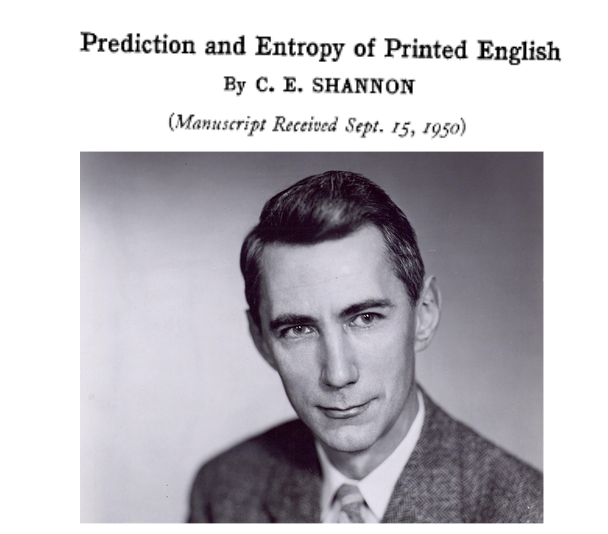
\includegraphics[scale = 0.4]{pics/shannon.png}
    \caption{Imagen de Shannon.}
    \label{fig:shannon}
\end{figure}

Por otro lado, en su libro \textit{Syntactic Structures} (1957), Noam Chomsky (en la Figura~\ref{fig:chomsky}), un lingüista y científico cognitivo, cuestionó la capacidad de los modelos de lenguaje probabilísticos para capturar y comprender la gramática del lenguaje humano \cite{chomsky2009syntactic}. Según Chomsky, la noción de ``gramaticamente correcto'' no puede ser equiparada a ``significativo'' en un sentido probabilista. Para ilustrar esto, presentó dos oraciones ficticias, ambas carentes de sentido:

\begin{enumerate}
    \item Colorless green ideas sleep furiously.
    \item Furiously sleep ideas green colorless.
\end{enumerate}

Aunque ambas oraciones carecen de significado, Chomsky argumentó que solo la primera se considera gramaticalmente correcta por los hablantes de inglés. Además, enfatizó que la corecctitud gramatical en inglés no puede determinarse únicamente mediante aproximaciones estadísticas. Aunque es poco probable que ninguna de las dos oraciones (1) o (2) haya surgido en documentos escritos en inglés, un modelo estadístico como los modelos de lenguaje vistos en este capítulo las consideraría igualmente ``remotas'' en relación al inglés. Sin embargo, la oración (1) es gramaticalmente correcta, mientras que la oración (2) no lo es, lo que destaca las limitaciones de los enfoques estadísticos para capturar la gramática. Estos argumentos retrasaron el estudio de los modelos de lenguaje probabilísticos durante varios años \cite{JurafskyBook}.

\begin{figure}[h]
    \centering
    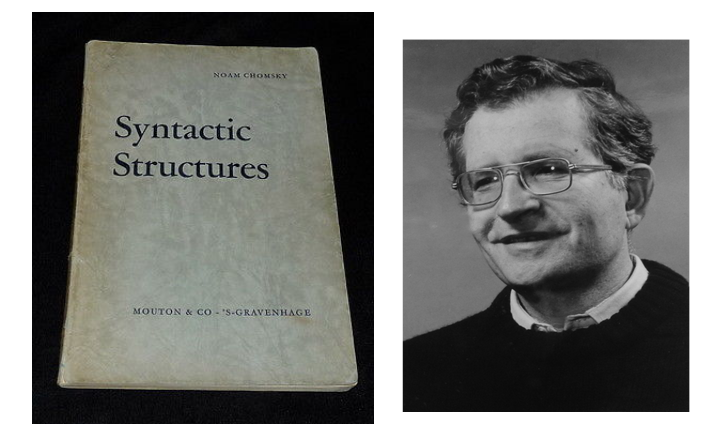
\includegraphics[scale = 0.4]{pics/chomsky.png}
    \caption{Imagen de Chomsky}
    \label{fig:chomsky}
\end{figure}


\section{Conclusiones}
La derivación de probabilidades en modelos de lenguaje probabilísticos implica tres pasos:
    \begin{enumerate}
        \item Expandir $p(w_1, w_2, \ldots, w_n)$ usando la regla de la Cadena.
        \item Aplicar los supuestos Independencia de Markov \\
        $p(w_i | w_1, w_2, \ldots, w_{i-2}, w_{i-1}) = p(w_i | w_{i-2}, w_{i-1})$.
        \item Suavizar las estimaciones utilizando conteos de orden inferior.
    \end{enumerate}
    
No obstante, los modelos de lenguaje de bigramas o trigramas (que consideran dos palabras anteriores como contexto) tienen limitaciones en contextos largos y no pueden aprovechar contextos similares. Por ejemplo, consideremos los contextos:
\begin{itemize}
 \item $c_1$: Después de comer cereales
\item  $c_2$: Luego de desayunar avena 
\end{itemize}

Aunque esperaríamos que las distribuciones de probabilidad $p(w|c_1)$ y $p(w|c_2)$ fueran similares, dado que $c_1$ y $c_2$ casi no comparten palabras, los modelos de n-gramas que se limitan a contar frecuencia de palabras no pueden capturar estas similitudes entre contextos.
    
    
Otros métodos para mejorar los modelos de lenguaje incluyen introducir variables latentes para representar tópicos, conocidos como modelos de tópicos \cite{blei2003latent} presentados en el Capítulo~\ref{cap_ir}. O alternativamente, reemplazar $p(w_i | w_1, w_2, \ldots, w_{i-2}, w_{i-1})$ con una red neuronal predictiva y una ``capa de embedding'' para representar mejor contextos más grandes y aprovechar similitudes entre palabras en el contexto. \cite{bengio2000neural}

Los modelos de lenguaje modernos utilizan redes neuronales profundas en su estructura principal y tienen un vasto espacio de parámetros como se verá en el Capítulo~\ref{cap_llm}.


\bibliography{bio}
\bibliographystyle{apalike}

\end{document}
